\chapter{Teoretická část studentské práce}

\section{Virtuální realita}

Virtuální realita (VR) je technologie, umožňující uživateli interagovat se simulovaným prostředím. Jde o vytváření vizuálního, sluchového, hmatového či jiného vjemu, budícího subjektivní dojem skutečnosti pomocí počítače, speciální audiovizuální helmy, brýlí popřípadě obleku.

\subsection{Stereoskopie}

Za nejjednodušší VR se dá považovat stereoskopie, což je technika vytváření 3D vjemu pomocí dvou 2D obrazů.


Stereoskopie využívá přirozené vlastnosti člověka, tzv. binokulárního vidění. To znamená, že se obrazy vnímané simultánně oběma očima spojí v jeden a navíc nám umožňuje vnímat hloubku prostoru. Každé oko vidí obraz mírně posunutý a mozek poté vytvoří na základě těchto vjemů 3D obraz. Existuje určité procento lidí, u kterých tato schopnost není vyvinuta a ti nejsou schopni správně 3D obraz vidět.


Tradiční stereoskopie vytváří 3D iluzi pomocí dvou 2D obrazů, s různými perspektivami téhož objektu, které se příliš neliší od toho, co by oči přirozeně viděly. Tím vlastně donutí mozek tyto dva rozdílné obrazy zpracovat jako v realitě a mozek vytvoří iluzi prostorového vidění.




\subsubsection{Anaglyf}

Je to technika, která nám umožňuje vytvářet stereoskopický obraz. Obraz pro každé oko je na tomtéž displeji, ale je v opačném odstínu, typicky červené a azurové. Pozorovatel má pak brýle, které mají barevné filtry a tak každé oko vidí pouze jeden z obrazů.

Nevýhodou tohoto řešení je ztráta barevné informace, protože pomocí ní je zakódovaná hloubka obrazu.

\subsubsection{Polarizace}

Další způsob zobrazení stereo obrazu je pomocí polarizačních brýlí. Tyto brýle mají polarizaci jednoho oka kolmou proti druhému. Obraz se pak zobrazuje nebo promítá střídavě přes dvě polarizační skla a brýle pak tyto obrazy odseparují.

Nevýhodou tohoto řešení je nedokonalá polarizace, která plně neodfiltruje druhý obraz a tak vznikají artefakty v obraze.

\subsubsection{Aktivní zatmívací brýle}

Tento způsob pracuje na principu multiplexování. Brýle, synchronně s displejem nebo projektorem, střídavě přepínají obraz pro obě oči.

Nevýhodou tohoto způsobu je velká cena.

\subsubsection{LCD brýle}

Toto jsou brýle, které mají 2 displeje, na které se promítají jednotlivé obrazy. Tyto brýle nemění svůj obraz při pohybu hlavou, jsou vhodné například pro 3D filmy. Brýle, které podporují sledování pohybu se řadí již do headsetů.

Nevýhodou této technologie je vysoká cena, zahřívání a nutné propojení kabelem.

\subsection{Headsety Virtuální reality}

\subsubsection{VFX1}

\begin{figure}
	\centering
	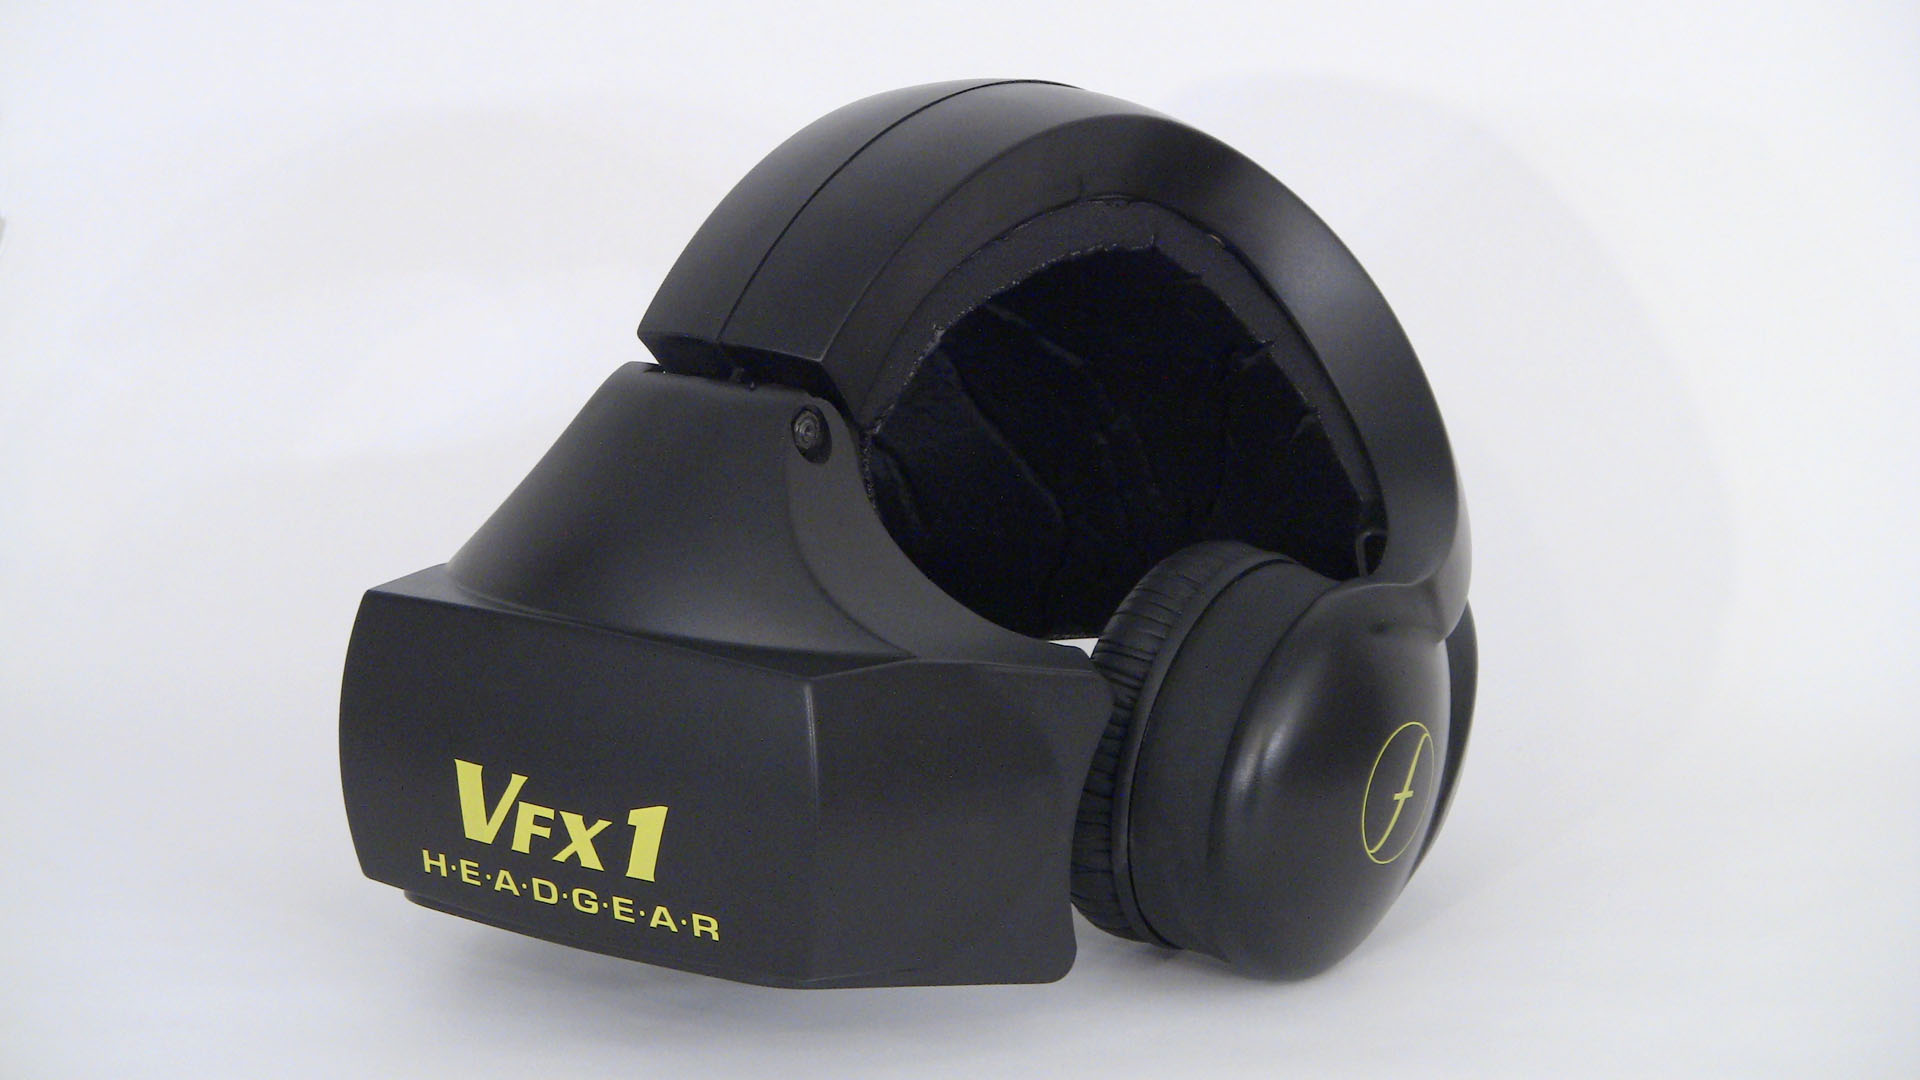
\includegraphics[keepaspectratio,width=\textwidth]{obrazky/vfx1}
	\captionof{figure}{VFX1 headgear}
\end{figure}

Za první komerční headset se dá považovat VFX1. Byl prodáván v devadesátých letech. Skládal se z helmy, ovladače a ISA karty.

Tento headset měl dva LCD displeje s rozlišením 263x230 a zorný úhel 45$ ^{\circ} $.\cite{vfx1}

\subsubsection{HTC Vive}

\begin{figure}
	\centering
	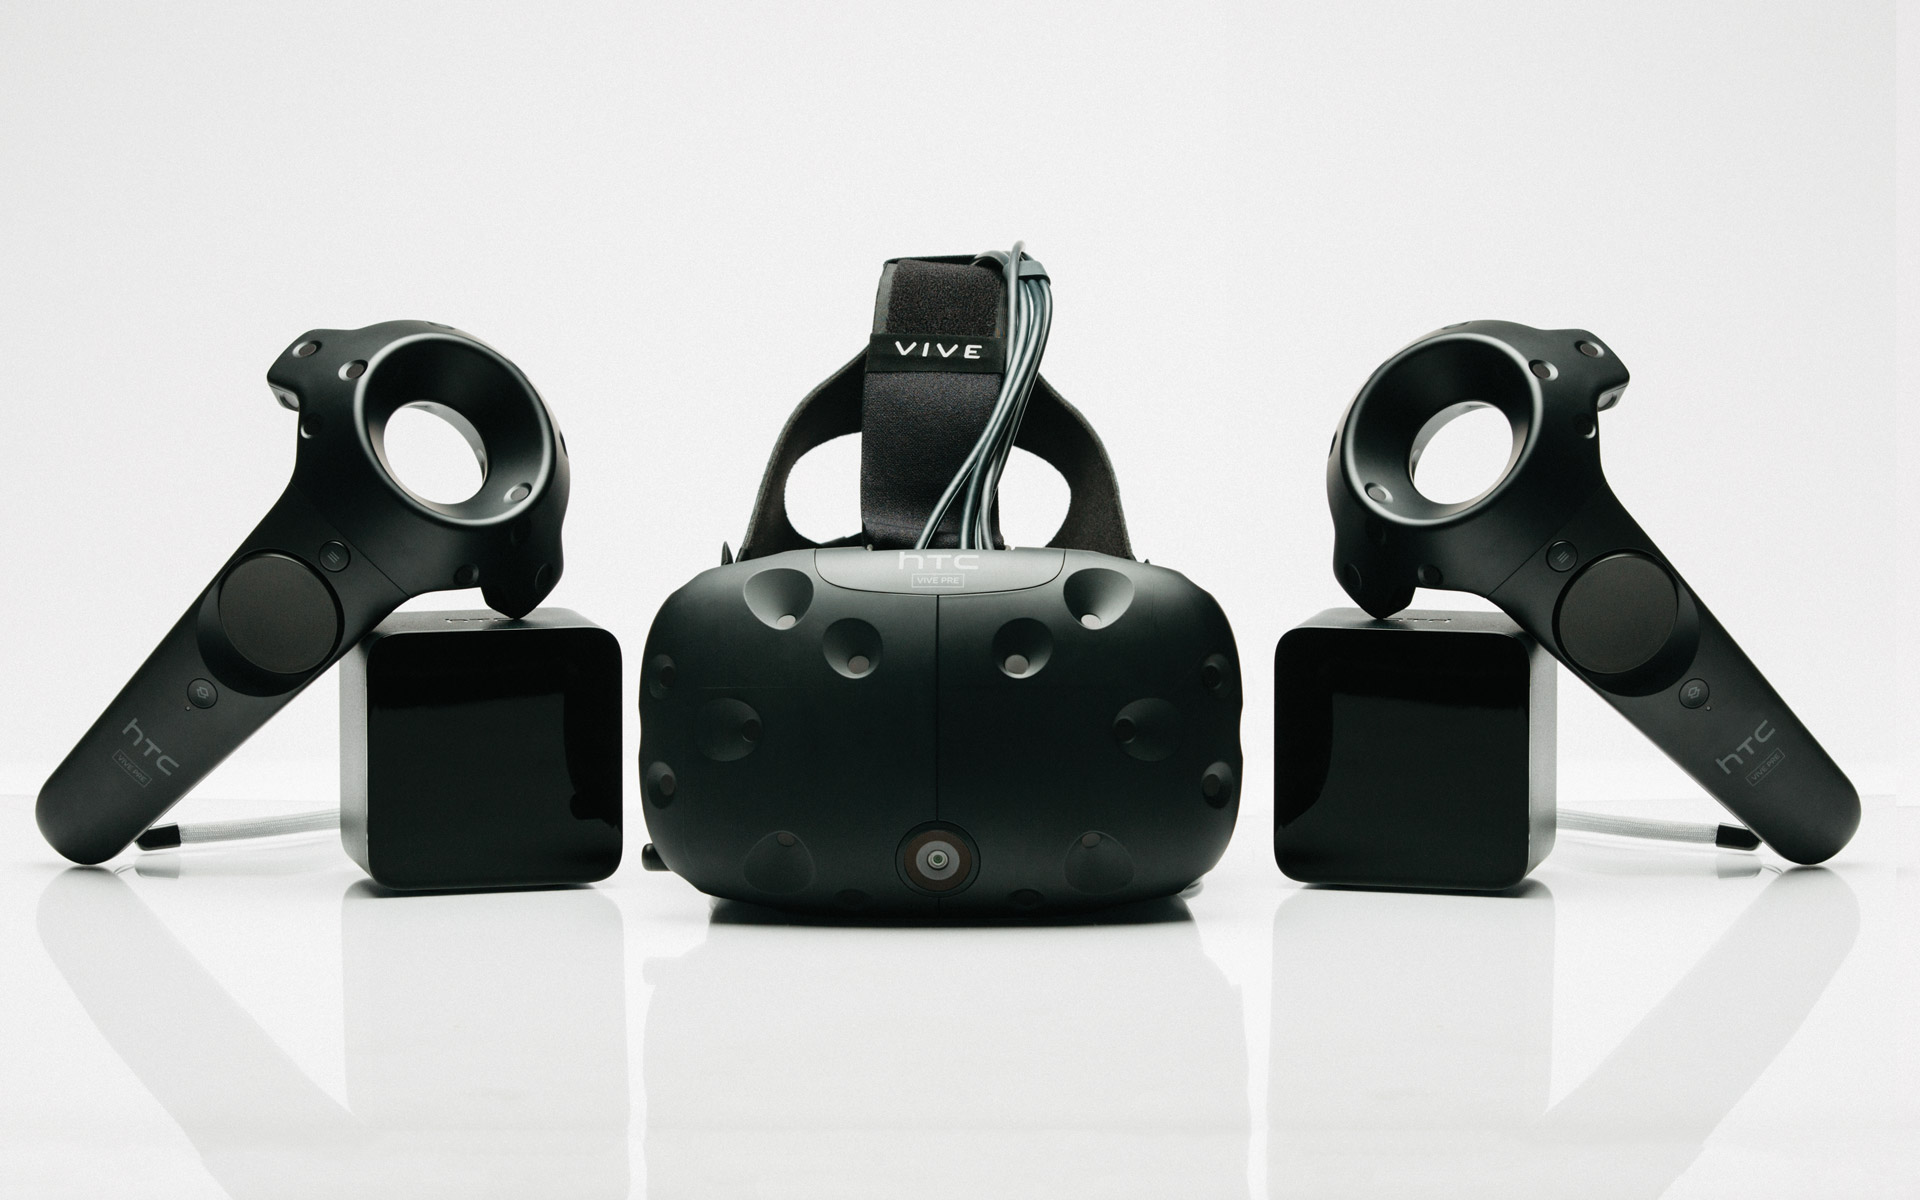
\includegraphics[keepaspectratio,width=\textwidth]{obrazky/vive}
	\captionof{figure}{HTC Vive}
\end{figure}

HTC Vive je headset pro virtuální realitu, vyvinut firmou HTC a Valve Corporation, byl vydán 5. dubna 2016. Tato sada obsahuje headset, dva prostorově sledované ovladače a dva snímače polohy. Uživatel se může pohybovat po místnosti velikosti 4.6\jedn{m} na 4.6\jedn{m}.\cite{vive_bbc}


HTC Vive využívá dva displeje s rozlišením 1080x1200\cite{vive_gamespot} a obnovovací frekvencí 90Hz. Zařízení používá více než 70 senzorů jako jsou gyroskopy, akcelerometry a laserové snímače.\cite{vive_bbc}\cite{vive-lasery} Kamera na přední straně headsetu pomáhá identifikovat objekty před uživatelem a zabrání tak kolizi.

Tento headset je podporován platformou SteamVR, vyvíjenou společností Valve Corporation.

\subsubsection{Oculus Rift}

\begin{figure}
	\centering
	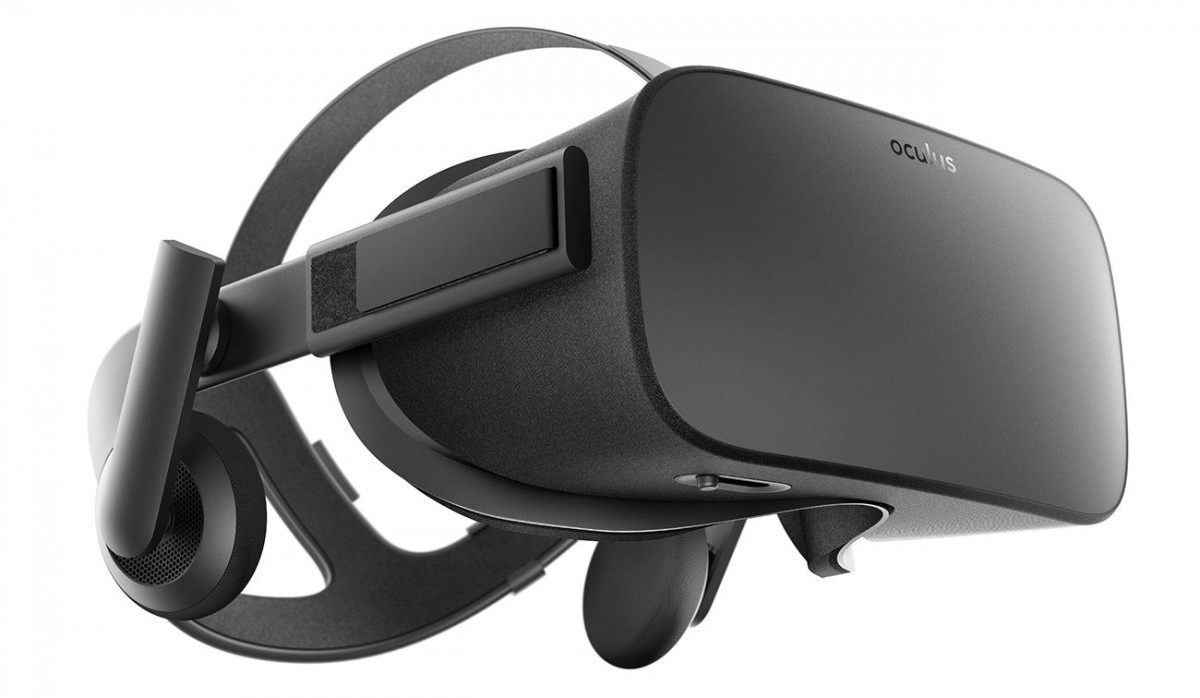
\includegraphics[keepaspectratio,width=\textwidth]{obrazky/oculus}
	\captionof{figure}{Oculus Rift}
\end{figure}

Oculus Rift je headset od společnosti Oculus VR, vydaný 28.3.2016.

Oculus Rift používá dva displeje s rozlišením 1080x1200, obnovovací frekvencí 90Hz a zorným úhlem 110$ ^{\circ} $.\cite{oculus_rift}. Navíc má zabudovaná i sluchátka. Pozice je sledována kromě akcelerometrů a gyroskopů také pomocí stacionární IR kamery, která snímá IR světla na headsetu a kompenzuje chyby inerciální jednotky v headsetu.

Oculus Rift je podporován Oculus Runtime a Steam VR.

\section{Možnosti programování zařízení pro VR}

Všecha tato zařízení pro svou funkci vyžadují, aby daný program s nimi komunikoval pomocí speciálního API.

Současný trh je velmi roztříštěný, každý výrobce headsetu má vlastní API a runtime, navzájem nekompatibilní. Tuto situaci se snaží zlepšit Valve, které vyvinulo OpenVR API primárně pro Vive a nabádá ostatní výrobce, aby dodali podporu jejich zařízení. OpenVR již podporuje Oculus, Vive a OSVR.

Jako další ohlásila vývoj jednotného API organizace Khronos, jejímž cílem je vyvinout API, které nahradí API všech výrobců a tím ulehčí práci vývojářů aplikací. Zároveň by se i zlevnil vývoj aplikací a rozšířil se okruh potenciálních zákazníků.  Valve již ohlásila, že do tohoto projektu předává své rozhraní OpenVR. \cite{khronos_vr}

Já mám k dispozici Vive a Oculus, výběr mých možností se proto zúží na:


\begin{itemize}
	\item Unity 3D, což je multiplatformní herní engine vyvinutý společností Unity Technologies. Tento engine podporuje všechny současné headsety. 
	
	\item Unreal Engine, multiplatformní herní engine vyvinutý společností Epic games. Tento engine podporuje všechny současné headsety.	
	
	\item Použít OpenVR C++ API a naprogramovat si vlastní aplikaci od základu.
\end{itemize}

Herní engine ulehčuje práci vývojářům, protože za ně řeší základní funkce všech her, např. kolize objetků, grafické efekty a v našem případě řeší i přístup k headsetu, tím pádem se mohou zaměřit více na samotný obsah hry. Na herní engine jsou kladeny jiné nároky, než na mou aplikaci. Geometrická náročnost modelu je u většiny her je podstatně menší než u mračna bodů, které potřebuji zpracovávat já. Naopak využívají fotorealistické efekty, mapř. různé odlesky, efekty osvětlení, které já nevyužiju.
Herní engine neobsahují algoritmy, které se využívají při práci s mračny bodů. Případné rozšíření funkcionality by bylo velmi náročné. Enginy používají vysokoúrovňové skriptovací jazyky, které nejsou primárně optimalizovány pro rychlost. Takže by se mohlo stát, že v případě přidávání dalších funkcí bych mohl narazit na limity schopností těchto enginů.
Dalším problémem by mohlo být přidávání knihoven. 
Herní enginy mají navíc licenční podmínky, které by nás mohly limitovat. Proto jsem zvolil cestu naprogramování vlastního enginu.